\begin{frame}
\frametitle{HES: Hypertext Editing System}
\begin{itemize}
	\item IBM/360 Model 50 mainframe
	\item online production of printed documents and the exploration of the hypertext concept
\end{itemize}

\begin{figure}[htbp]
	\centering
	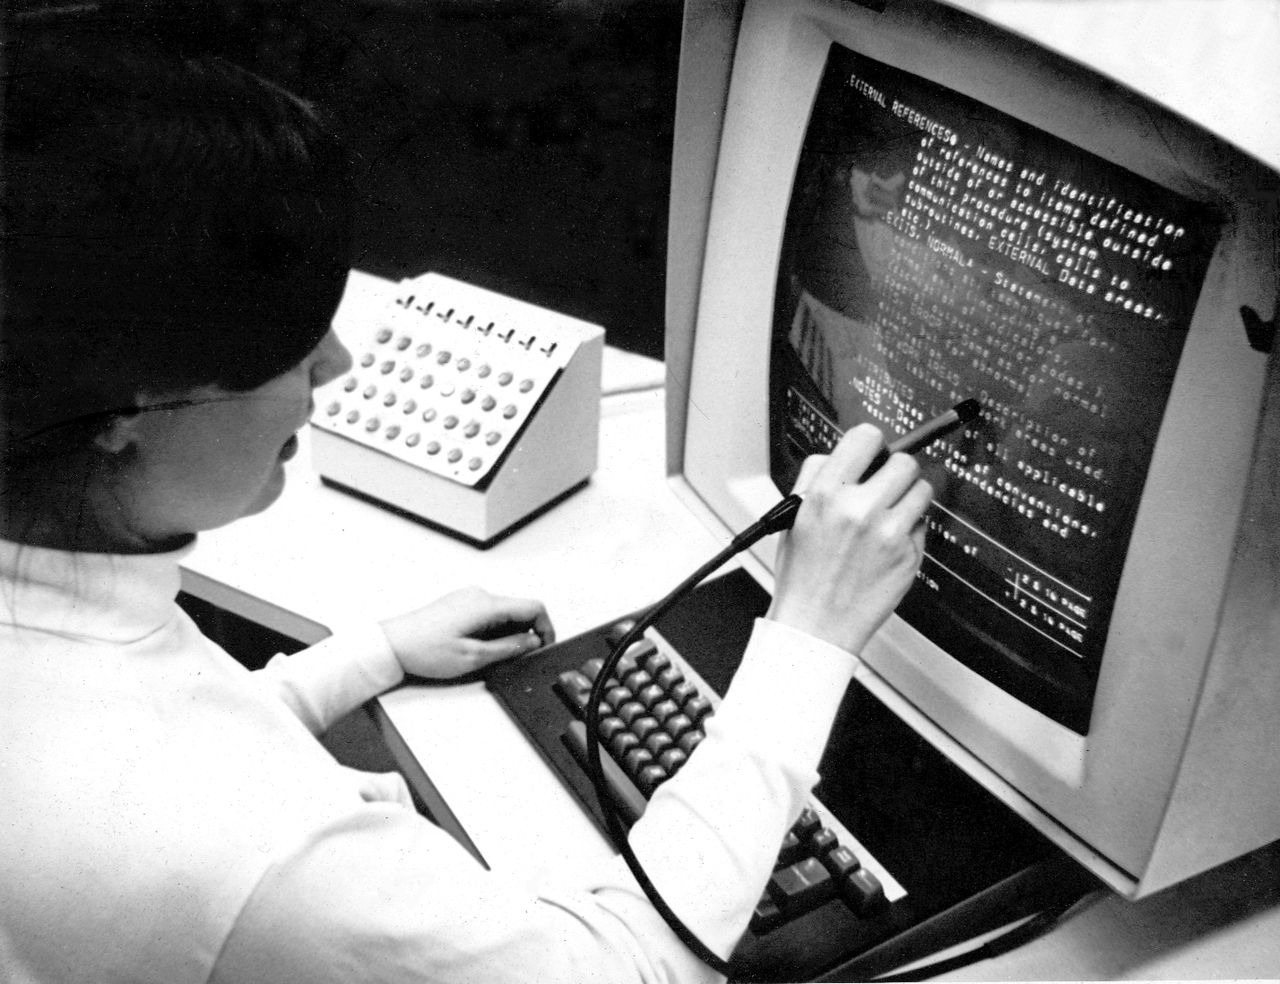
\includegraphics[width=0.50\textwidth]{images/hes}
\end{figure}

\end{frame}

\begin{frame}
\frametitle{HES: Hypertext Editing System}
\framesubtitle{Funktionen}
\begin{itemize}

	\item Invisible control information allows the printing of the entire hypertext in linear form
	\item pointer manipulation to text fragments
	\item If one instance of text is modified the changed text will show up in all other places as well [Yankelovich et al. 85, p. 23]
	

\end{itemize}
\end{frame}

\begin{frame}
\frametitle{FRESS: File Retrieval and Editing System}
\framesubtitle{Funktionen}

	\begin{itemize}
		\item windows
		\item tag: one-way link
		\item jumps: bi-directional links
		\item backtrack through a sequence of links
	\end{itemize}

\end{frame}
